\documentclass[nobib]{tufte-handout}

\newcommand{\bra}[1]{\left(#1\right)}
\usepackage{hyperref}
\usepackage[activate={true,nocompatibility},final,tracking=true,kerning=true,spacing=true,factor=1100,stretch=10,shrink=10]{microtype}
\usepackage{color}

% Set up the images/graphics package
\usepackage{graphicx}
\setkeys{Gin}{width=\linewidth,totalheight=\textheight,keepaspectratio}

\title{Notes for POL 23700 - Modern Weapons And International Relations}
\author[Zeke Ulrich]{Zeke Ulrich}
\date{\today}  % if the \date{} command is left out, the current date will be used

% The following package makes prettier tables.  We're all about the bling!
\usepackage{booktabs}

% The units package provides nice, non-stacked fractions and better spacing
% for units.
\usepackage{units}

% The fancyvrb package lets us customize the formatting of verbatim
% environments.  We use a slightly smaller font.
\usepackage{fancyvrb}
\fvset{fontsize=\normalsize}

% Small sections of multiple columns
\usepackage{multicol}

% These commands are used to pretty-print LaTeX commands
\newcommand{\doccmd}[1]{\texttt{\textbackslash#1}}% command name -- adds backslash automatically
\newcommand{\docopt}[1]{\ensuremath{\langle}\textrm{\textit{#1}}\ensuremath{\rangle}}% optional command argument
\newcommand{\docarg}[1]{\textrm{\textit{#1}}}% (required) command argument
\newenvironment{docspec}{\begin{quote}\noindent}{\end{quote}}% command specification environment
\newcommand{\docenv}[1]{\textsf{#1}}% environment name
\newcommand{\docpkg}[1]{\texttt{#1}}% package name
\newcommand{\doccls}[1]{\texttt{#1}}% document class name
\newcommand{\docclsopt}[1]{\texttt{#1}}% document class option name

% Define a custom command for definitions
\newcommand{\defn}[2]{\noindent\textbf{#1}:\ #2}

% Define graphics path
\graphicspath{ {./images/} }

\begin{document}

\maketitle

\begin{abstract}
These are lecture notes for fall 2023 POL 23700 at Purdue.
\end{abstract}

\tableofcontents

\section{Course Introduction}
This course introduces the student to the roles that modern weapons systems 
play in contemporary international relations.
\\~\\
Learning objectives: 
\begin{enumerate}
    \item Identify and explain the elements and requirements of nuclear deterrence.
    \item Discuss the role of technology in the emergence of modern total warfare.
    \item Analyze the impact of contemporary information technologies on the conduct of warfare.
\end{enumerate}

\pagebreak 

\section{Military revolutions}
\defn{RMA}{Revolution in military affairs. A major change in warfare brought about by a new application of technology.}
\defn{Total war}{The full mobilization of a country for the war effort, where 
the entire economy, social organization, and civil population become dedicated 
to the war effort.}

Technology is the great equalizer. Whereas historically
power was held by trained warriors and those who 
commanded them, the democratization of force through 
modern war machines enables a nineteen-year-old boot camp 
graduate to have the same effect on the battlefield
as a soldier with decades of experience. 

The five most important RMAs are, in chronological order:
\begin{enumerate}
    \item The gunpowder revolution
    \item The Napoleonic revolution
    \item The industrial revolution
    \item The airpower revolution
    \item The nuclear revolution
\end{enumerate}
In general, these things are true of RMAs:
\begin{itemize}
    \item They involve new technologies
    \item Technology is not limited to Weapons
    \item Strategic competition encourages military innovation
    \item Innovation in warfare is driven by the basic struggle of defense vs offense
    \item RMAs are driver by technology, which is self-accelerating. Thus each RMA occurs faster than the previous
\end{itemize}

\begin{marginfigure}
    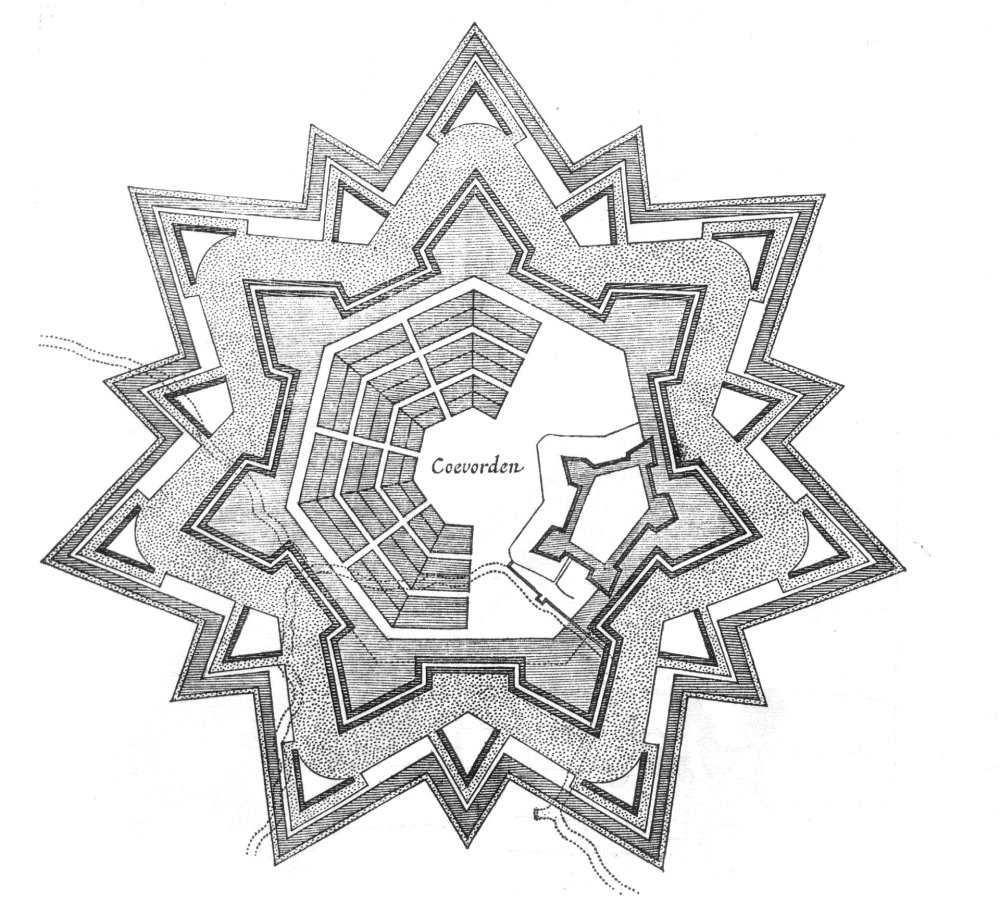
\includegraphics{Coevorden.jpg}
    \caption{Bastion fort}
    \label{bastion}
\end{marginfigure}
\marginpar{
    The bastion fort was a very flat structure composed of 
    many triangular bastions, specifically designed to cover each 
    other. To counteract cannonballs, defensive 
    walls were made stouter.
}

\subsection{The gunpowder revolution}
The gunpowder revolution lasted from the 1400s to the 1700s.
Prior political power was decentralized amongst 
smaller localities. In Europe, these smaller localities were hundreds of lords 
guided by the overarching influence of the Catholic church. Defense had the advantage. 
Sieges could last months or years, allowing the defenders an ever-present option to retreat. 
Knights were the dominant power. The more numerous footmen were untrained peasants 
pressed into service by nobles. Between the 1400s and 1850 consolidated countries emerged,
largely thanks to newly invented cannons capable of destroying castle walls. 
Defensive attempts to mitigate the destructive power of cannons, such as bastion forts, were expensive
and rare. Now that cannons were able to easily destroy castles, 
royalty needed a strong, constant military force to protect themselves. 
These trained armies were able to combat the poorly organized feudal knights 
and led to the solidification of nation states. Feudal states, independent cities, 
and religious enclaves had no ability to forward standing armies and were conquered 
and assimilated. The battlefield advantage shifted from skilled knights to
masses of peasants taught to hold a gun straight and fire on command. 
Discipline became more important than skill. Lines of riflemen 
faced off, firing and firing again 
until enough musket balls had found their mark that the opposing line 
fell. 

As states with these larger armies assimilated their 
neighbors, Europe as we know it today began 
to emerge. Power solidified within families 
and individuals, and the medieval era of loose organization 
was supplanted by one of tighter regulation and control. 

\subsection{The Napoleonic revolution}

When Napoleon emerged as a great leader, the world 
experienced true nationalism for the first time. No 
longer did the poor need to be pressed into service, 
but now could be coerced in service of a greater cause. 
These patriotic soldiers were more motivated and 
their compatriots at home more willing to support 
the war. Citizens of French towns began thinking of 
themselves as French citizens, and national pride 
began to spread outwards from France. Napoleon structured his 
army into self-sufficient and purpose-built corps who supported 
one another. He promoted based on skill, improved logistics, 
and conquered large swathes of Europe before his enemies learned 
to adopt or counter his tactics. Angered by French conquest, 
nationalism flared in Prussia, Spain, and Britain and 
the disjoint European nations banded together to oppose the 
superiority of Napoleonic France. We thus learn an important lesson:
good technology is adopted by everyone, eventually reducing the 
exclusivity its inventors at first enjoy. This lesson repeats itself 
in every RMA we will study. 

\subsection{The industrial revolution}

The industrial revolution allowed for the first true instance of total war, 
as states centralized after the Napoleonic wars became able to direct 
output and civilian population to drive large-scale wars. Three important 
technologies emerged under the industrial revolution:
\begin{itemize}
    \item The railroad
    \item The telegraph
    \item The rifle
\end{itemize}
These innovations will be crucial going forward. Railroads allowed 
the mass transit of supplies and troops across land, allowing massive 
and rapid mobilization and effectively bringing countries closer together. 
Speed and response time became much more important once an enemy army could travel across 
several countries in the span of hours. Efficient and timely execution of 
orders necessitated efficient and timely communication of orders, 
which came with the invention of the telegraph. The telegraph sped 
up war even farther and shifted the advantage to the first mover in a war,
such as the Prussians in the wars of German reunification. 

Now, let's look at the final crucial invention: the rifle. 
Old muskets took half a minute to load under the best conditions, 
malfunctioned twenty-five percent of the time, and had 
an accurate range of around one hundred meters. Newly 
invented percussion rifles could kill at a mile, was much 
more reliable, and once repeating rifles were invented, 
soldiers could fire dozens of rounds per minute. The logical 
conclusion of this accelerating firing speed was the machine gun, 
capable of firing hundreds of rounds per minute. 
While the gunpowder revolution made firearms possible, 
each one had to be hand made and assembled. The processes 
of the industrial revolution made guns cheaper and faster, 
making guns accessible, interchangeable, and more common. 

The tinderbox of heavily armed, nationalist European states 
was quick to ignite when the Serbian assassination of Austrian archduke 
Franz Ferdinand sparked WWI. Military thinkers of the time 
saw the success of the wars of German reunification 
and believed that victory would favor those who struck first.
The Germans planned, in the event of war, to strike France 
by bypassing its defense through Belgium, then shifting 
attention to the lethargic beast of Russia, before fending 
off any attack from Great Britain, who would be threatened 
by the proximity of Belgian ports to the English coastline. 
After Franz Ferdinand's assassination, Germany struck first
and launched an invasion of Belgium. Thanks to the railroad 
and telegram, France was able to quickly mobilize inwards and 
repel the German invasion miles outside of Paris. While fleeing, 
Germans turned around, dug trenches, set up machine guns, 
and fired backwards on the advancing French forces. Unable 
to advance, French and German forces tried to outflank 
one another, lengthening the trenches until they spanned the entire country. 
Nationalism drove thousands of young enlists to the trenches, 
where they shot one another with mass-produced rifles. 
Movement at the trenches stalled, causalities mounted, 
and poison gas floated across no-man's land to dissolve the 
lungs of young recruits. Primitive airplanes were unable to 
advance the front, and progress seemed impossible until 
the invention of modern warfare's most iconic children: 
the tank. 

The tank, along with the entry of the United States late 
in the war, broke through the German lines. Germany was routed 
as the tank could survive the machine gun and small-arms 
fire in no man's land, travel over difficult terrain, 
crush barbed wire, and cross trenches to assault 
fortified enemy positions with powerful armament. However, 
technology again diffused, and by WWII every major country had 
adopted this powerful war machine, again equalizing the 
battlefield. Germany's WWII Blitzkrieg doctrine combined intensive training,
wireless radio communication, and novel tactics, allowing it 
to steamroll Poland and France. The Nazis used radio communication to 
exploit weaknesses in enemy lines, create holes, push through, 
and respond rapidly. 

\subsection{The airpower revolution}

During the Combined Bomber Offensive from 1943 
to 1945, the U.S. faced the problem of needing 
a fighter with the range to escort bombers deep
into German industrial areas. This need was met 
with the deployment of the P-51 Mustang in large 
numbers in the winter of 1943/44, allowing the 
combination of B-17 bombers and P-51 fighters 
to achieve air superiority and expand bombing 
capabilities. The tonnage of bombs dropped 
increased dramatically over the years, from 31 
tons in 1939 to 525,000 tons in 1944, with a 
reduction to 190,000 tons in 1945 as Germany 
surrendered in June.

In the years 1944-45, there were constant 
attacks on German industrial and population 
centers, leading to the leveling of cities 
through raids that used both explosive and 
incendiary bombs. Attacks on railroads aimed 
to prevent troops and supplies from reaching 
the Western front. The bombing of Dresden in 
April 1945 was particularly devastating, and 
Germany surrendered two months later.

Despite the heavy bombing, there was little 
evidence that it reduced German morale, as 
there was no sign of diminished will to fight, 
similar to the British experience during the 
Battle of Britain. Although some downplayed 
the role of the Combined Bomber Offensive by 
pointing out that German industrial output 
grew in 1944, targeting transportation and 
oil was critical and forced Germany to divert 
resources. 

While strategic bombing certainly contributed 
to the German defeat, its decisiveness is 
debated, as air power alone did not bring 
victory. The campaign raised moral issues by 
blurring the distinction between civilian and 
military targets, resulting in total war where 
civilian casualties greatly outnumbered military 
ones.

\subsection{The nuclear revolution}

\defn{Nuclear triad}{Nuclear weapons deployable 
from air (bombers), land (missles), and sea (submarines)}

The prevailing theory during the nuclear age 
was that mutually assured destruction would 
ensure the Cold War stayed cold. The potential 
of overwhelming nuclear destruction would deter 
the US and the USSR from attacking one another, 
ensuring no wars on a scale comparable to the 
World Wars would break out. This is debated:
other researchers believe that the world was 
relatively peaceful because the memory of WWII
was fresh in the memory of the globe. The United 
States, with its Marshall plan, rebuilt Europe 
at a cost of tens of billions of dollars and wasn't 
eager to have to re-rebuild. People learned 
that war was destructive, war was pointless, 
and war robbed millions of their lives. Another 
competing theory is that Soviet ideology was 
cautious, since Marxist communism expected 
that capitalist societies would destroy themselves 
internally. Personally, I believe any 
one of these reasons fails to tell the whole story. 
The true reason nuclear war didn't erupt is 
likely due to some combination of the above, luck, 
and reasons unknown to the public. 

Traditional deterrence doesn't apply to non-state 
actors. If a terrorist faction was to obtain 
nuclear weapons, they have no return address 
for a retaliatory strike. In addition, when 
someone is willing to give up their life 
nuclear deterrence doesn't hold much weight 
anyway. 

\subsection{The Iraq War}

After the invasion of Iraq in 2003, it was confirmed that Iraq
did not have weapons of mass destruction (WMD) that could be used 
against the United States, as was previously reported. 
Saddam Hussein had no connections to Al Queada, and the war 
cost trillions of dollars, thousands of US lives, and hundreds 
of thousands of Iraqi lives. In retrospect the war was a clear 
mistake, but intelligence of the era strongly suggested that 
the Iraqis did have WMD and that war was justified. It was 
only after the fog of war was lifted that this falsehood was 
disproven. Its veracity aside, the argument that Hussein had nuclear, 
chemical, or biological weapons of mass destruction and was 
too unpredictable to be left alone was the primary justification 
for America's invasion of Iraq. The influential vice president 
of the time, Dick Cheney, subscribed to what was known as the 
\emph{one percent doctrine}, the idea that if there was even a 
one percent chance that Iraq had nuclear weapons, the US must
invade for the safety of its citizens and for its allies. The 
was concern that, in addition to a direct attack from Saddam, 
WMD would be passed off to Iraqi proxy groups who would use them
against US interests. 

Not everyone was on board with the Iraq war. Then just as now, 
the war was extremely controversial. One argument against 
the war was that Saddam Hussein may be evil, but he wasn't insane, 
and traditional nuclear deterrents would be effective against him. 
It was argued that Iraq's invasion of Kuwait 
was logical, since Iraq had "protected" Kuwait 
from Iran and incurred heavy debt. Prominent scholar 
John Mearsheimer argues that Saddam was not 
suicidally crazy given that he held power for four 
decades. The ends justify the means type beat. 
Additionally, he only used conventional weaponry 
against Western nations in the Gulf War. Saddam had 
used chemical and biological weapons against enemies 
without the ability to deter him, which shows a 
certain amount of rationality. Moreover, the US had previously 
aided Saddam's regime in developing biological 
weapons to counter Iranian and Russian influence. 
The US had felt comfortable giving Saddam weapons 
in the past because he hated Al-Qaeda and any 
suspicion for a terror attack would fall on him. 
Previous analysis had concluded that Saddam would 
not sacrifice his life or regime for terrorism, 
and thus with the clarity of hindsight we might 
conclude that traditional nuclear deterrence would 
have been effective and there was no need for an
invasion of Iraq. 

\subsection{Terrorism}

\defn{Terror group}{Non-state actor who wish to achieve a politcal 
objective by attacking non-military targets.} 

Terrorists want 
attention and employ shock value as an integral part of their 
strategy. This may not include mass casualties (e.g. IRA calling 
ahead to warn of imminent bombings), but many groups do aim 
to inflict death on large scales (e.g. ISIS, Al-Qaeda, Aum Shinrikyo). 
Intent is concerning, but the terrorist groups that make headlines 
are those with both intent and capability to inflict terror. 
Many groups whose aim is to kill on a mass scale would love 
to have weapons of mass destruction, e.g. nuclear weapons, biological 
weapons, or chemical weapons. Lucky for the rest of us, refining 
uranium is costly and difficult, putting nuclear weapons out of the 
reach of even the most powerful groups. Stealing a nuke is similarly, 
if not more, difficult. The other two, unfortunately, are well within 
the grasp of ordinary people. While we won't dive into the details on 
how to manufacture either chemical or biological 
weapons\footnote{Fester, Uncle. 1997. Silent Death. Loompanics Unlimited.}, 
in this class we classify chemical agents into three categories. 
\begin{itemize}
    \item Choking agents: attack the lungs or respiratory system, 
    producing asphyxia. Examples include phosgene, chlorine. 
    \item Blistering agents. Creates severe chemical burns 
    through contact with the skin. Examples include mustard gas. 
    \item Nerve agents. Attacks the body's nervous 
    system. Spreads through contact or inhalation. 
    Death by asphyxiation or cardiac arrest may 
    follow in minutes due to the loss of the body's 
    control over respiratory and other muscles. Examples include sarin, VX, 
    and Novichok. 
\end{itemize}
These weapons are best used for area denial. 
While making these weapons is relatively 
simple, deploying them effectively
is often more expensive and less destructive than 
conventional methods like car bombings. 
If you have a bunch of people packed together 
closely in an enclosed space, the ideal scenario 
for a chemical weapon, a bomb could still cause 
more harm. While chemical weapons have been used 
and their effects are horrific, in terms of number 
of causalities conventional methods have a superior 
track record. Biological agents are similarly 
inefficient. While many have attempted to leverage 
biological warfare in service of their goals, 
few have determined that its effect is greater 
than the effect of traditional terrorism. 

\subsection{Information Revolution}
We are arguably in the midst of a new revolution 
in military affairs, marked by the use of precision munitions, 
intelligence gathering, reducing the fog of war, 
and the computerization of command, control, and 
communications. Decisions are now more informed 
than ever before, with decisions being relayed quickly and 
over vast distances. This RMA is most noticeable in 
airpower, although it affects every aspect of war. 
This, along with the associated improvements 
in and reliance on technology, has changed the 
model of warfare from full mobilization to a central 
core of highly trained full-time soldiers extending 
their influence with information and remote operations. 
This RMA has its roots in the Cold War, where the US 
and its NATO allies acknowledged that Russia was 
capable of fielding a massive swarm of soldiers 
and it would be difficult to defeat them by numbers alone. 
The idea behind the information revolution is 
to leverage information to increase the effectiveness 
of efforts. 

\end{document}